\section{Experiments and Results}

\subsection{Protocol and exploratory statistics}

ASR and audio-conditioned grounding use all 471 valid files. Parse failures and out-of-bounds coordinates remain incorrect. Click transitions are CC (both correct), WC (raw wrong, corrected-run correct), CW (raw correct, corrected-run wrong), and WW (both wrong). Frozen counts are primary. Exact two-sided sign tests on WC/CW, Wilson intervals, command-clustered bootstraps, and identical-prompt UI-TARS reruns were added post hoc. The reported sign-test $p$-values are exploratory, unadjusted for multiple comparisons, and calculated at audio-item level despite repeated renditions per command; they do not establish confirmatory or causal effects.

\subsection{ASR performance}

Both ASR systems return records for all 471 files (Table~\ref{tab:asr}). Whisper has lower CER/WER on this audio. Code-switched CER is 10.02 percent for Whisper and 22.03 for Typhoon. Literal LER is 45.90 percent (28/61 audio-level instances) and 96.72 percent (59/61), respectively. These 61 instances derive from only 18 commands. Equivalent Thai-script transliterations may contribute to literal LER, but that explanation has not been established by an exhaustive lexical audit; lexical errors, script differences, and omissions have not been separated.

\begin{table}[t]
\centering
\caption{ASR performance (percent; $n=471$ each). LER is over 61 audio-level loanword instances.}
\label{tab:asr}
\small
\begin{tabular}{lrrrr}
\toprule
ASR & CER & WER & LER & Fail \\
\midrule
Whisper large-v3 & 5.55 & 10.72 & 45.90 & 0.00 \\
Typhoon ASR & 6.95 & 13.27 & 96.72 & 0.00 \\
\bottomrule
\end{tabular}
\end{table}


\subsection{Gold text versus raw ASR}

GPT-5.5 parses every baseline output, with pooled click accuracy of 76.56 percent on gold, 75.80 on Whisper, and 76.43 on Typhoon text (Table~\ref{tab:grounding}). UI-TARS scores 44.53/39.07/40.34 percent and has 9/34/29 parse failures, respectively. Its pooled point-in-image rates remain below 92 percent. Gold accuracy is reported separately by tier: GPT-5.5 T4 is 62.50 percent, whereas its raw-ASR T4 scores are 58.33--59.17 percent. Neither value establishes a model ceiling.

Gold uses 128 commands and ASR conditions use 471 correlated renditions. Existing paired bootstraps average ASR click correctness within command, subtract that command's gold score, and resample 128 commands (10,000 draws; seed 20260719). The GPT-5.5 Whisper/Typhoon mean differences are $-0.52$/$+0.07$ points, with 95 percent intervals $[-3.12,+2.02]$/$[-2.34,+2.86]$; UI-TARS differences are $-4.43$/$-3.32$, with intervals $[-12.50,+3.71]$/$[-10.87,+4.36]$. There is no detectable gold-versus-ASR difference. Small underlying effects, robustness to ASR errors, and insufficient benchmark sensitivity or power remain possible.

\begin{table*}[t]
\centering
\caption{Baseline grounding (percent). Click includes failures; PFail is parse-failure rate. Gold has 32 commands per tier; each ASR condition has 111 T1 and 120 T2--T4 audio items. Tier scores are condition-specific, not model ceilings.}
\label{tab:grounding}
\small
\begin{tabular}{llrrrrrrr}
\toprule
Model & Transcript & $n$ & Click & PFail & T1 & T2 & T3 & T4 \\
\midrule
GPT-5.5 & Gold & 128 & 76.56 & 0.00 & 100.00 & 71.88 & 71.88 & 62.50 \\
GPT-5.5 & Whisper & 471 & 75.80 & 0.00 & 100.00 & 73.33 & 72.50 & 59.17 \\
GPT-5.5 & Typhoon & 471 & 76.43 & 0.00 & 100.00 & 75.83 & 73.33 & 58.33 \\
UI-TARS & Gold & 128 & 44.53 & 7.03 & 75.00 & 34.38 & 43.75 & 25.00 \\
UI-TARS & Whisper & 471 & 39.07 & 7.22 & 70.27 & 29.17 & 29.17 & 30.00 \\
UI-TARS & Typhoon & 471 & 40.34 & 6.16 & 56.76 & 41.67 & 40.83 & 23.33 \\
\bottomrule
\end{tabular}
\end{table*}


\subsection{Transcript changes and pooled clicks}

Table~\ref{tab:correction} separates literal transcript metrics from observed pooled click differences. Typhoon A/B are complete no-op controls. Under the post-hoc normalization rule, all 72 Whisper A changes and 63 of 72 B changes are cosmetic. B has nine normalized-CER recoveries and no normalized false corrections. C has 38 Whisper and 48 Typhoon normalized false corrections. Thus large literal A/B false-correction rates mostly reflect normalization mismatch; normalized counts also remain metric-based, rather than direct semantic-error rates.

Pooled click differences are mixed and mostly negative, but independent reruns prevent causal attribution to correction. In particular, the UI-TARS/Typhoon/A no-op differs by $-6.16$ points despite identical transcript text. Figure~\ref{fig:correction-tier} retains the tier variation and negative differences; its literal FCR must be interpreted alongside the cosmetic-change diagnostic.

\begin{table*}[t]
\centering
\caption{Literal transcript metrics (percent; shared across grounders) and observed pooled click differences (percentage points). FCR includes cosmetic changes; net is recovery count minus false-correction count. Click differences compare independent runs. W/T denote Whisper/Typhoon.}
\label{tab:correction}
\small
\begin{tabular}{llrrrrrr}
\toprule
ASR & Method & Changed & Recovery & FCR & Net & GPT-5.5 $\Delta$ & UI-TARS $\Delta$ \\
\midrule
W & A & 15.29 & 0.00 & 15.29 & -72 & -0.64 & +0.21 \\
W & B & 15.29 & 0.64 & 15.29 & -69 & -0.42 & -1.70 \\
W & C & 23.99 & 1.70 & 23.35 & -102 & -1.91 & -4.03 \\
T & A & 0.00 & 0.00 & 0.00 & 0 & -1.27 & -6.16 \\
T & B & 0.00 & 0.00 & 0.00 & 0 & -0.85 & -0.21 \\
T & C & 11.25 & 3.18 & 10.19 & -33 & -1.27 & -1.49 \\
\bottomrule
\end{tabular}
\end{table*}


\begin{figure*}[t]
    \centering
    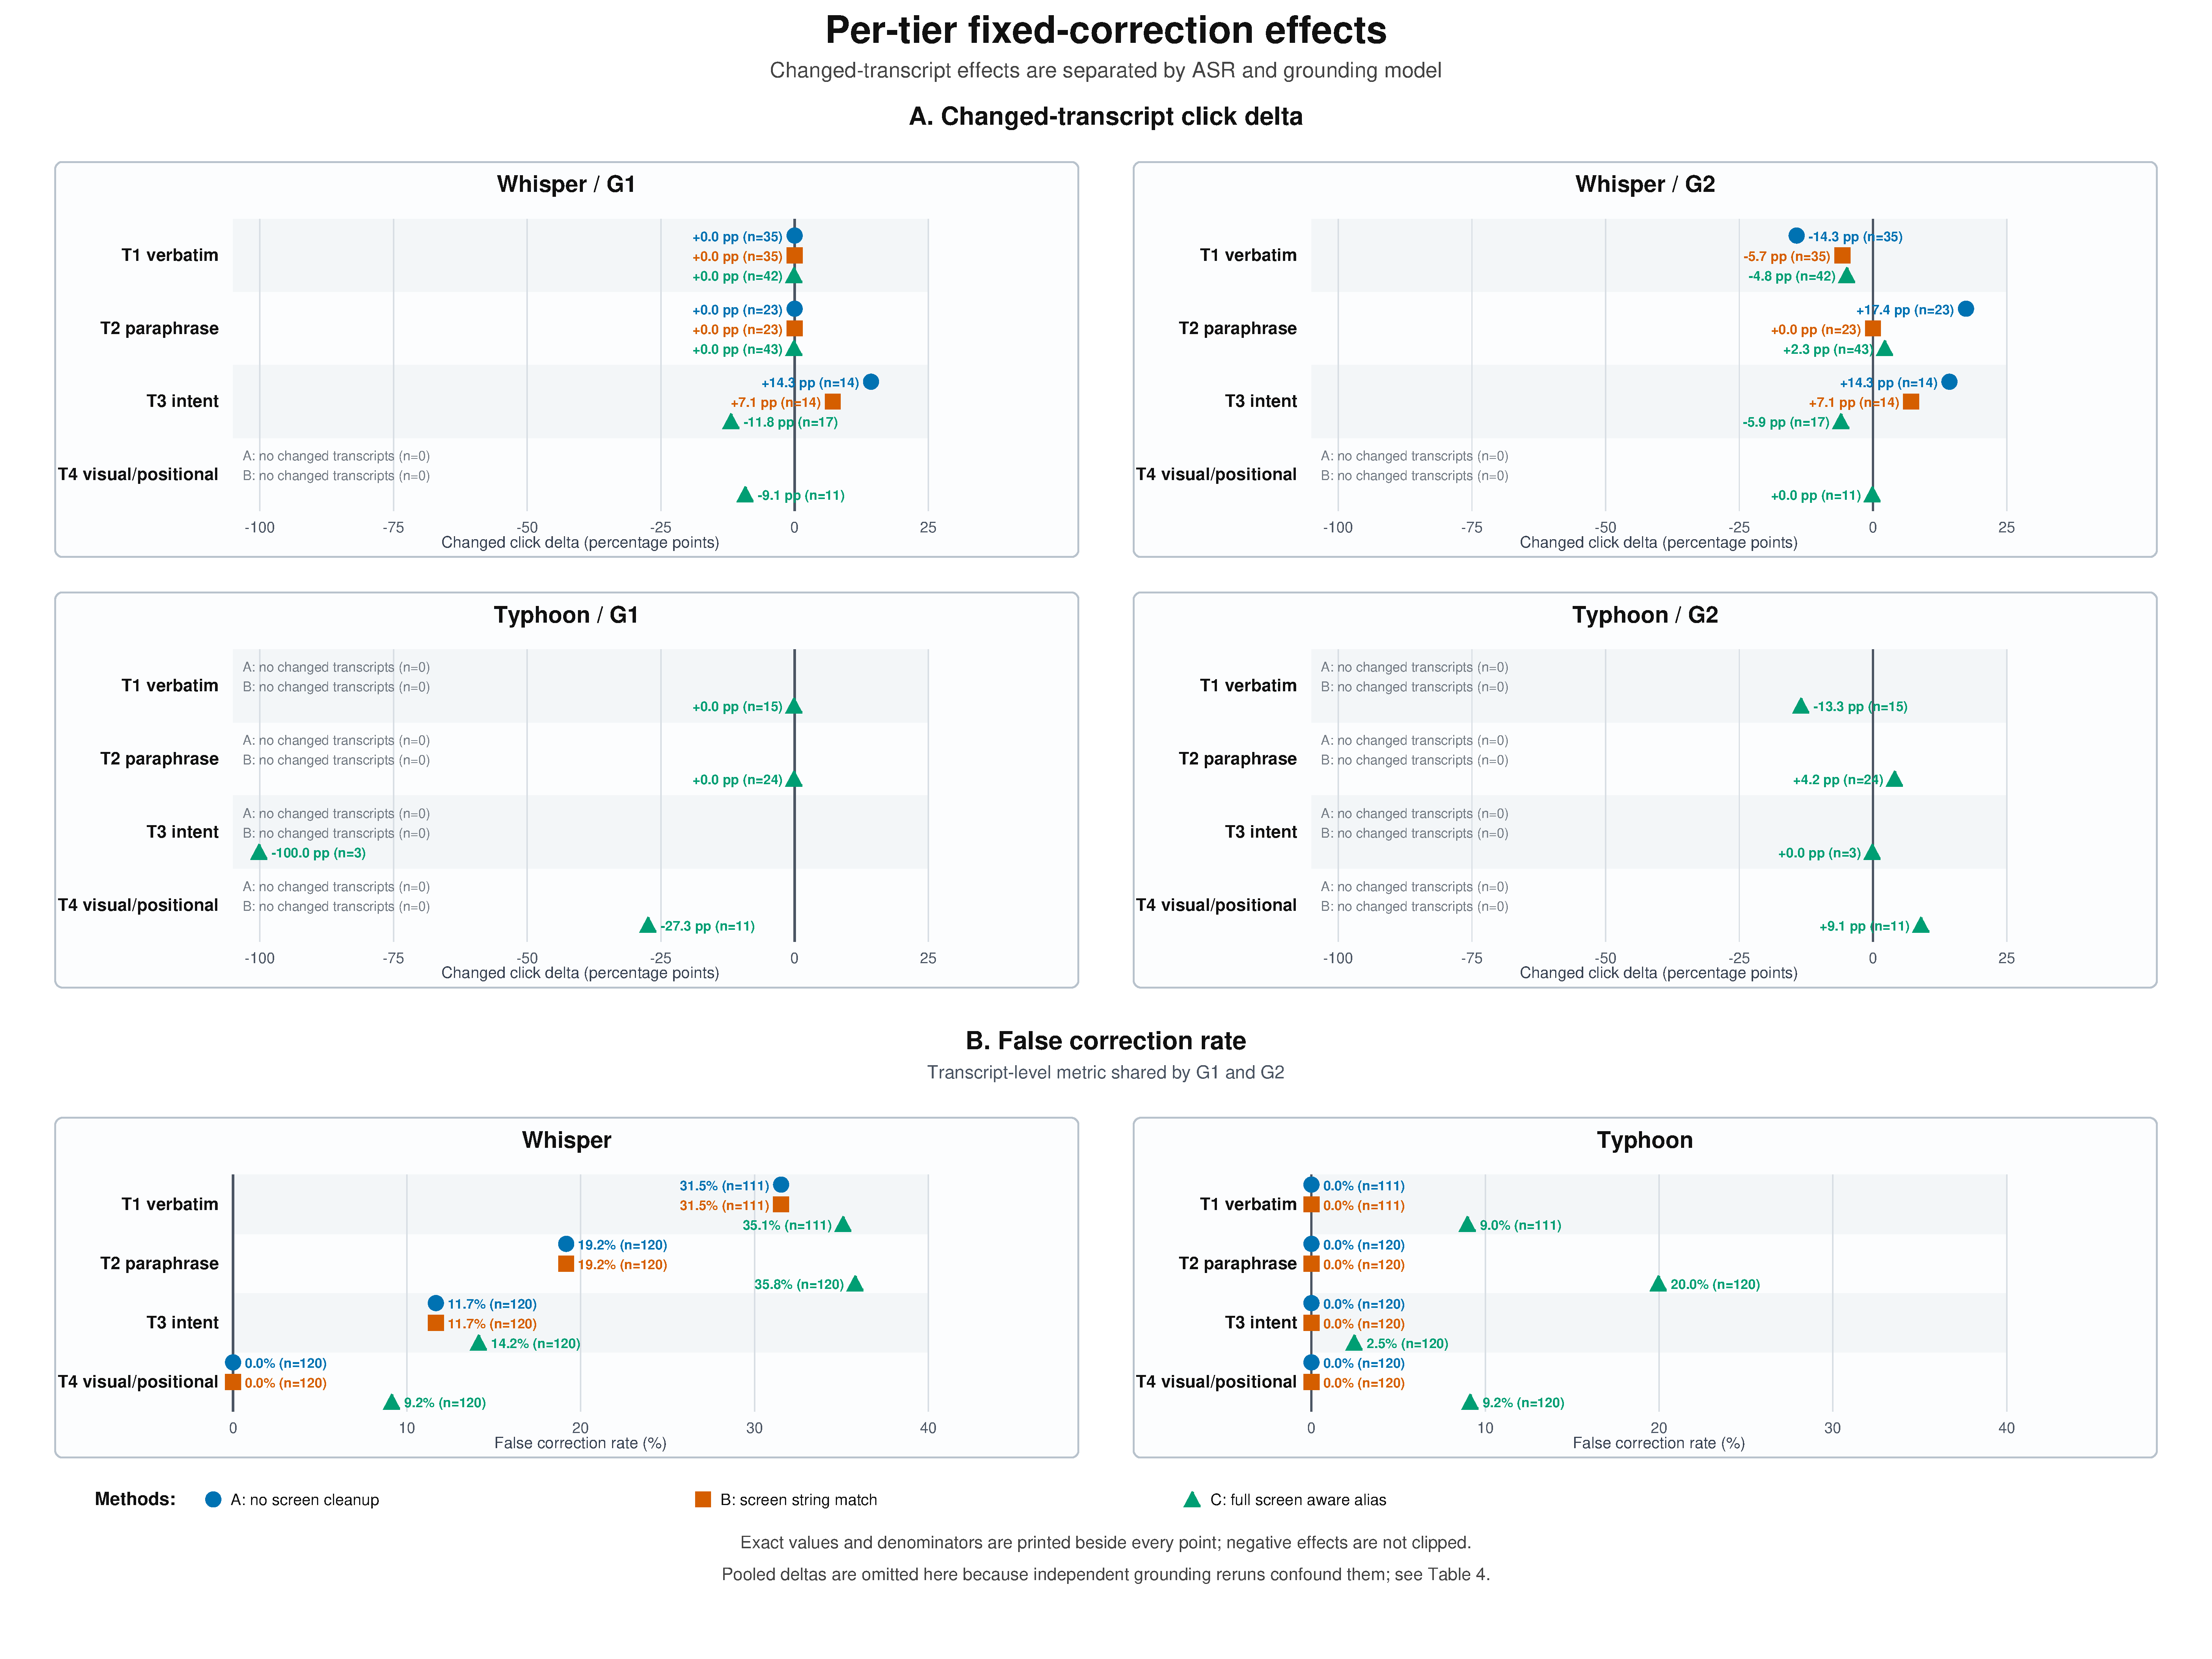
\includegraphics[width=\textwidth]{figures/figure2_per_tier_correction_effects.pdf}
    \caption{Observed per-tier changed-transcript click differences and literal false-correction rate (FCR), using the frozen figure data. Artwork uses ``effects'' for cross-run differences, not causal estimates. FCR is string-based and includes cosmetic changes. Table~\ref{tab:changed-unchanged} reports unchanged/no-op comparisons. G1/G2 denote GPT-5.5/UI-TARS.}
    \label{fig:correction-tier}
\end{figure*}

\subsection{Changed, unchanged, and rerun comparisons}

For GPT-5.5/Whisper, A/B changed-subset differences of $+2.78$/$+1.39$ points reflect only two/one net WC flips (exploratory $p=0.50/1.0$; Table~\ref{tab:changed-unchanged}). GPT-5.5/Typhoon/C shows an adverse difference in one exploratory comparison: $-11.32$ points among 53 changed items, WC=0 and CW=6, with unadjusted post-hoc $p=0.03125$. The six deteriorations arise from \emph{three unique commands}, not six independent commands. Repeated renditions, multiple testing, and separate inference runs preclude a general claim that C degrades performance. GPT-5.5/Whisper/C differs by $-2.65$ points ($p=0.375$).

UI-TARS changed-subset WC/CW counts are nearly balanced. Its Typhoon/A no-op has WC=49 and CW=78 ($p=0.0127$, subject to the same exploratory caveats). The existing identical-prompt rerun of all three raw UI-TARS conditions changes click correctness on 25--27 percent of items and parse status on 10--11 percent. Exact coordinates recur for only 1--5 items per condition. Net gold/Whisper/Typhoon differences are $+3.13$/$+0.21$/$-0.64$ points. These records demonstrate rerun variability but neither remove it from corrected-versus-raw comparisons nor establish serving-system drift.

\begin{table*}[t]
\centering
\caption{Observed changed versus unchanged click differences. Independent runs do not isolate correction causality. Deltas are percentage points. Same-U is exact coordinate repeatability among unchanged prompts. A dash means no transcript changed.}
\label{tab:changed-unchanged}
\small
\begin{tabular}{lllrrrrr}
\toprule
Grounding & ASR & Method & $n_C$ & $\Delta_C$ & $n_U$ & $\Delta_U$ & Same-U \\
\midrule
GPT-5.5 & W & A & 72 & +2.78 & 399 & -1.25 & 279/399 \\
GPT-5.5 & W & B & 72 & +1.39 & 399 & -0.75 & 277/399 \\
GPT-5.5 & W & C & 113 & -2.65 & 358 & -1.68 & 247/358 \\
GPT-5.5 & T & A & 0 & -- & 471 & -1.27 & 333/471 \\
GPT-5.5 & T & B & 0 & -- & 471 & -0.85 & 332/471 \\
GPT-5.5 & T & C & 53 & -11.32 & 418 & 0.00 & 278/418 \\
UI-TARS & W & A & 72 & +1.39 & 399 & 0.00 & 5/399 \\
UI-TARS & W & B & 72 & -1.39 & 399 & -1.75 & 3/399 \\
UI-TARS & W & C & 113 & -1.77 & 358 & -4.75 & 1/358 \\
UI-TARS & T & A & 0 & -- & 471 & -6.16 & 2/471 \\
UI-TARS & T & B & 0 & -- & 471 & -0.21 & 5/471 \\
UI-TARS & T & C & 53 & 0.00 & 418 & -1.67 & 4/418 \\
\bottomrule
\end{tabular}
\end{table*}


\subsection{Manual review and qualitative cases}

One human reviewer coded 140 deterministically selected cases using the saved review guide. Selection covered failures, correction transitions, no-op changes, loanwords, and T3/T4 difficulties, then balanced tier and model/method groups; each tier contributes 35 cases. This is a purposive stratified sample, not a prevalence sample. The reviewer saw system identities, gold targets/text, automatic candidate categories, predicted coordinates, and click outcomes. Coding was unblinded and assigned one final category with evidence notes per case. Inter-reviewer agreement was not measured; between-reviewer disagreement resolution was inapplicable.

The guide includes lexical/segmentation errors, confusable labels, visual/positional failures, ambiguity, over-correction, parse/out-of-bounds failures, transcript/click transitions, and unchanged-prompt variability. The largest sampled categories are variability (27), confusable labels (16), positional failures (16), parse failures (15), and ambiguous instructions (14). These counts cannot estimate benchmark-wide ambiguity or identify its contribution to total error.

Case 093 (shopping\_002, T2) replaces a Thai basket expression with \emph{Cart} and coincides with WC for UI-TARS/Typhoon/C. Case 135 (settings\_004, T2) inserts unsupported \emph{Notifications} into already-correct text and coincides with CW for UI-TARS/Whisper/C. Case 118 (mock\_finance\_001, T1) repairs \emph{Paybill} to \emph{Pay bill}, yet the UI-TARS/Whisper/B click becomes wrong. In Case 003 (mock\_finance\_003, T2), unchanged Typhoon text accompanies GPT-5.5/A moving from \emph{History} to the correct \emph{Statements} target. These are qualitative associations, not isolated correction effects; full records and the guide accompany the package.

\subsection{Native-format probe and reproducibility}

The existing post-hoc UI-TARS native-template probe used all 34 G2/Whisper parse failures plus 66 randomly sampled remaining items (seed 20260719), on the same July 19 serving stack. Of the 34 failures, native formatting parses 23 and clicks correctly on 14. Among the other 66 items, shared JSON parses 66 with 30 correct clicks; native formatting parses 45 with 21 correct. Totals are 66 versus 68 parsed and 30 versus 35 correct out of 100. This failure-enriched, nonrepresentative probe does not establish protocol fairness or full-benchmark native-format performance. The exact template, parser, sampled IDs, and outputs are retained.

\paragraph{Data and code}
The versioned benchmark and reproducibility package, including frozen data, predictions, exact prompts, aliases, thresholds, review records, and available serving configurations, is available at \url{https://github.com/paphanin/ThaiVoice-GUIBench/releases/tag/v1.0.0}. Historical vLLM/CUDA versions, hardware, complete server launch flags, and local decoding defaults were not recorded and cannot be reconstructed reliably.

